\chapter{Introduction}

\textbf{Author: Ida Hönigmann}

\vspace{2mm}

Robots are getting more and more mobile. While a few years ago their usage was mostly limited to aid factory automation, robots have found widespread adoption in a multitude of industries, such as self driving cars and autonomous delivery drones.
A challenge frequently encountered is navigating in unknown environments, which either requires the robot to sense specific characteristics of its surroundings or to communicate with some external system.

The problem of navigation has been looked at from many different angles. One popular approach in mobile robotics is to use the GPS, an external positioning system. In order to determine the position of a robot using the GPS, it has to establish communication with at least four satellites. The exact position of each satellite as well as the current time is broadcast by the satellites. By measuring the time needed for the signal to reach the robot, the position can be calculated up to three meters accurately.

However, in some cases positioning a robot using external positioning methods is not possible. In the case of the GPS this can be due to obstacles interfering with the radio signals send by the satellites, for example occurring inside a building. In comparison this work focuses on a system that can navigate in outdoor as well as in indoor environments. 

\section{Goal}
The goal of this diploma thesis is to implement a system which can localize a robot using no other sensors than a camera. This limitation was purposely chosen as the system will be used by future robotic students at the HTBLuVA (Technical Secondary College) and many robot systems used in the field of education are only poorly equipped with sensors that are able to detect its environment. One sensor used in the field of educational robotics is the either already equipped, or easily mountable camera.

As part of this thesis the authors not only want to implement an easy to use API for future robotic students, but to also show the possibilities and advantages of machine learning in localisation.

In order to accomplish precise localisation in various different surroundings, the authors plan on implementing a neural network. The neural network should take images, taken by the camera, as an input, and outputs the relative distance to any object shown in the images. By using machine learning the system should be less dependent on a specific situation or setup in comparison to different camera based localisation methods. For example the localisation should work on objects varying in size and shape, as well as in different situations of lighting.

\section{Motivation}
In July 2019 the two authors of this work participated in the aerial tournament at the Global Conference on Educational Robotics held in Norman, Oklahoma. One of the two main challenges encountered at this tournament was landing a drone next to some randomly placed object, which colour, shape and size was known in advance.

The second challenge the participants at the tournament faced was flying from one side of randomly placed cardboard boxes to the other. The cardboard boxes, representing a mountain, are placed in one of various configurations, one of which can be seen in figure~\ref{pic:introduction_motivation_mountain}.

\begin{figure}[h]
	\centering
	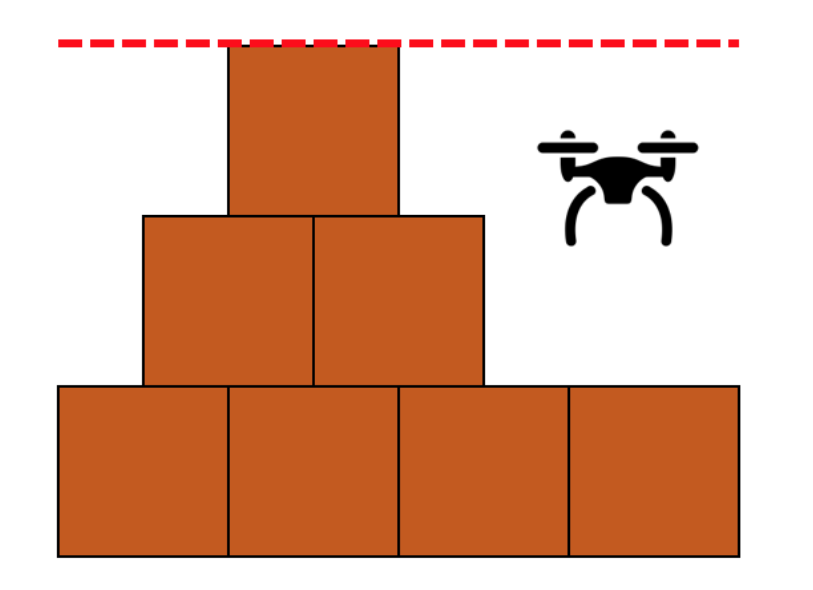
\includegraphics[width=2.5in]{img/introduction_motivation_mountain.png}
	\caption{Seven cardboard boxes, representing a mountain, are placed in a random configuration. The team scores points if the drone passes the mountain while staying under the height limit indicated by the red dotted line.}
	\label{pic:introduction_motivation_mountain}
\end{figure}

The drones used at this aerial tournament are equipped with a camera, while lacking any other sensor that can be used to detect the obstacles and game items. Therefore the participants needed to be able to detect the distance to the object and the cardboard boxes using only the camera. At the Global Conference on Educational Robotics the authors of this work decided to detect the object based on its colour, but had to invest quite some time tweaking the values to get the localisation working correctly. Therefore the authors want to research and implement a method that is more robust than the colour based one.

\section{Outlook / Perspective}
The objective of this work is to create a system which uses machine learning methods in localising objects. After having trained the system, it should reliably return the x, y and z distances to an object, shown in two pictures taken from different angles.

It is planned that the distance will be measured from the second camera position to the centre of object, as seen in Figure~\ref{pic:introduction_outlookPerspective_pointsOfView}.

\begin{figure}[h]
	\centering
	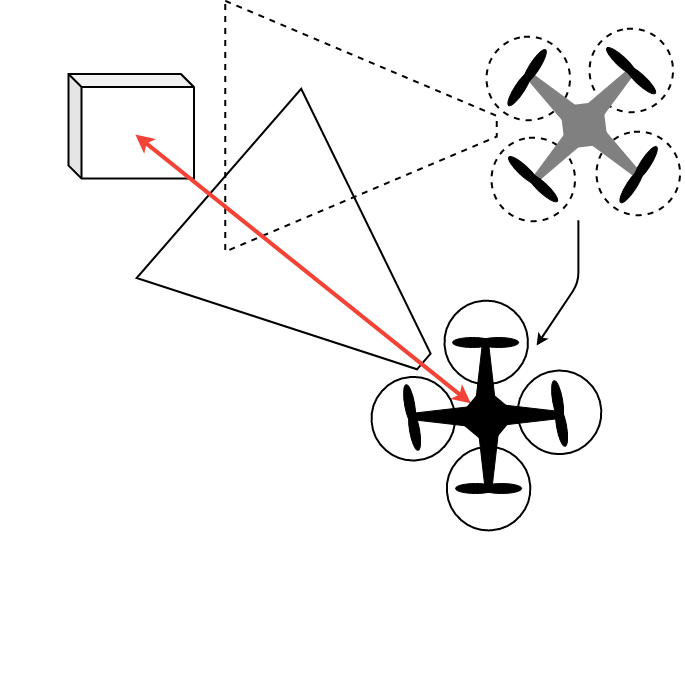
\includegraphics[width=3in]{img/introduction_outlookPerspective_pointsOfView.png}
	\caption{A drone tries to gather the data needed for the localisation of an object. After taking the first picture (dotted line) the drone flies to a second position (solid line) to take another picture from a different point of view. The red line indicates the distance vector to be returned.}
	\label{pic:introduction_outlookPerspective_pointsOfView}
\end{figure}

\section{Equipment}


[TODO: Mit welcher Drohne soll das System funktionieren?, Kamera auf der Drohne]

\filbreak
